\documentclass[a4paper,12pt]{report}
\usepackage[french]{babel}
\usepackage[utf8]{inputenc}
\usepackage[T1]{fontenc}
\usepackage[a4paper, top=2cm, bottom=2.5cm, left=2cm, right=2cm]{geometry}


\usepackage{graphicx}
\usepackage{caption}
\usepackage{subcaption}
\usepackage{lmodern}
\usepackage{parskip}
\usepackage{microtype}
\usepackage{enumitem}
\usepackage{booktabs}
\usepackage{tabularx}


\usepackage{hyperref}
\hypersetup{
    colorlinks=true,
    linkcolor= black,
    filecolor=magenta,      
    urlcolor=cyan,
    pdftitle={Overleaf Example},
    pdfpagemode=FullScreen,
}

\begin{document}
\begin{titlepage}
    \centering
    \vspace*{0.2cm} 
    

    
    % Optional logo
    
\includegraphics[width=0.5\textwidth]{upc.jpg}\par
    \vspace{1cm}

    
     \textbf{\Large Cahier des charges} \\[1em]
    \textquotedblleft \textsc{Projet de programmation} \textquotedblright \\[1em]
    \textbf{\large sujet} \\[1em]
    \rule{\textwidth}{0.4pt} \\[1em]
    \textbf{\LARGE
    Développement d’un système de recommandation basique } \\[1em]
    \rule{\textwidth}{0.4pt}

    \vspace{1.8cm}
    
    
    

\noindent
\begin{minipage}[t]{0.45\textwidth}
    \textbf{\large Réalisé par:} \\[1em]
    Dihya MEGHERFI \\
    Dina BOUDERKA \\
    Lilia JESOVER--ENGEL \\
    Adriana NGANZU NDAYIDI \\
    
\end{minipage}
\hfill
\begin{minipage}[t]{0.45\textwidth}
    \raggedleft
    \textbf{\large Encadré par:} \\[1em]
    M Enzo BONNEAU
\end{minipage}

    \vspace{1.2cm}
    
 \rule{\textwidth}{0.4pt} \\[1em]
    \textbf{\LARGE
    Année: 2025/2026}\\


   
    \vfill
\end{titlepage}

\newpage
\tableofcontents
\newpage



\chapter{Préambule}
Dans le cadre du projet de programmation de deuxième année de la licence d’informatique et applications, il nous est demandé de produire un système de recommandation basique. Nous avons choisi de concevoir un système capable de recommander des films à un utilisateur à partir d’un jeu de données et en utilisant un algorithme de recommandation. \\
Le but de ce cahier des charges est de définir les besoins, les fonctionnalités attendues ainsi que les contraintes du projet.


\chapter{Guide de lecture}

\section{Maîtrise d’œuvre}
La maîtrise d'œuvre caractérise l'équipe responsable de la réalisation du projet.
\subsection{Responsable}
La fonction de chef de projet est exercée à tour de rôle par les membres du groupe.
Le rôle du responsable est de :
\begin{itemize}
    \item Organiser les réunions
    \item Répartir les tâches
    \item Assurer le respect des délais
\end{itemize}
\subsection{Personnel administratif}
Le projet ne comporte pas de personnel administratif spécifique. Les membres du groupe assurent directement l’organisation et le suivi administratif.  
\subsection{Personnel technique}
Le personnel technique est constitué des membres du groupe projet.

Le rôle de l’équipe est d’assurer:

\begin{itemize}
\label{BE1}
    \item L’analyse du besoin
    \item Le développement du backend et du frontend
    \item Le traitement des données
    \item Les tests du système
    \item L’intégration des différentes parties du projet
\end{itemize}
\newpage
\section{Maîtrise d’ouvrage}
La maîtrise d'ouvrage caractérise la personne ou l'entité qui a demandé la création du produit.

La maîtrise d'ouvrage de ce projet est représentée par son
commanditaire, UFR Maths-info de l'Université Paris Cité et l'encadrant du projet, M. Enzo Bonneau.

Ce dernier a pour rôle de :

\begin{itemize}
    \item Valider les fonctionnalités majeures du produit
    \item Évaluer la conformité du produit final au cahier des charges
    \item Approuver le produit final
\end{itemize}


\chapter{Concepts de base}
\textbf{Système de recommandation :} \\
Un système de recommandation est un outil informatique permettant de proposer des éléments à un utilisateur en prédisant ses préférences, en se basant sur les notes qu’il attribue à d'autres éléments ainsi que les informations associées à ces derniers.

\textbf{Jeu de données (dataset):} \\
\label{JD1}
Le modèle s'appuie sur un jeu de données qui est un ensemble structuré d’informations. Dans ce projet, il contient des films avec leurs caractéristiques (titre, genre, note moyenne, réalisateur, année de sortie) ainsi que les notes attribuées par des utilisateurs.

\textbf{Recommandation basique}: \\
\label{algorec}
Ces données sont exploitées par un algorithme de recommandation basique consistant à générer des suggestions personnalisées pour chaque utilisateur en se basant sur les notes attribuées et les informations des films.

\textbf{Interface web:} \\
Partie visible de l’application permettant à l’utilisateur de consulter la liste de films, de donner ses notes et de recevoir les recommandations personnalisées générées par le système.




\chapter{Contexte}
Le projet s'inscrit dans le domaine du traitement des données et du développement d'applications de gestion. Avec l'augmentation constante du volume de contenus numériques, les utilisateurs sont confrontés à une surcharge d'informations qui rend difficile la découverte de contenus pertinents. Les systèmes de recommandation constituent une solution essentielle pour personnaliser l'expérience utilisateur en proposant des suggestions adaptées aux préférences individuelles.
Dans l'environnement actuel, où l'utilisateur est submergé par les contenus numériques, l'enjeu principal est de démontrer qu'il est possible, même avec des algorithmes simples, de filtrer efficacement l'information et de personnaliser l'expérience des utilisateurs. Le projet vise à développer un système de recommandation de films à partir d'un jeu de données.
Il permet également de comprendre les mécanismes fondamentaux des algorithmes de recommandation et de les appliquer dans une situation concrète. Il contribue à mobiliser et à développer des compétences en traitement de données, en programmation, ainsi qu'en conception d'une interface web interactive.

\chapter{Historique}
Depuis quelques années, le volume de contenus cinématographiques n’a cessé de croître. Cette croissance, initialement vue comme un avantage, a progressivement engendré une difficulté : la découverte de films pertinents est devenue de plus en plus difficile.\\
Quelque temps après, les systèmes de recommandation se sont progressivement imposés comme des outils essentiels dans les applications numériques modernes permettant de suggérer des contenus personnalisés grâce à des mécanismes de filtrage.\\
C’est dans ce contexte d’évolution des usages que ce projet a été initié. L’objectif est de concevoir un système de recommandation simple appliqué au domaine cinématographique.


\chapter{Description de la demande}

\section{Les objectifs}
\begin{itemize}
    \item Exploiter un jeu de données contenant des films.
    \item Développer un système de recommandations simple.
    \item Générer des recommandations personnalisées.
    \item Afficher clairement la liste de recommandations.
    \item Expliquer les recommandations produites.
    \item Mettre en place une interface web simple permettant à l'utilisateur d'interagir avec le système.
\end{itemize}

\section{Produit du projet}
Le produit est une application web autonome proposant un système basique de recommandation de films. À partir d'un jeu de données contenant des informations sur des films, l'application analyse les données disponibles afin de générer des suggestions adaptées aux préférences d'un utilisateur.
Le système repose sur une méthode simple de comparaison et permet de visualiser les recommandations produites à travers une interface interactive.

\section{Fonctionnalités du produit}
\label{fnct}
\subsection{Fonctionnalités obligatoires}
\begin{enumerate}[label=FR-0\arabic*, leftmargin=1.7cm]
    \item Système de recommandation basique
    \item Interface web fonctionnelle et interactive (voir les maquettes en annexe : \ref{fig:1})
    \item Création d'un compte utilisateur
    \item Authentification et connexion de l'utilisateur
    \item Choix des préférences utilisateur, pour amorcer le moteur de recommandation
    \item Génération d'une liste de films recommandés 
    \item Notation des films par l'utilisateur
    \item Affichage des informations d'un film
    \item Barre de recherche
\end{enumerate}
\subsection{Fonctionnalités optionnelles}
\begin{enumerate}[label=OFR-0\arabic*, leftmargin=1.7cm]
    \item Exclure de la recommandation les films déjà notés ou recommandés
    \item Justification de la recommandation
    \item Possibilité pour l'utilisateur de choisir les critères sur lesquels la recommandation va se baser (par exemple : le réalisateur, un acteur, un genre ...)
    \item Proposition de films « similaires à ... »
    
    \item Permettre à l'utilisateur de mettre un film en favoris
    \item Retour de l'utilisateur sur la recommandation
    \item Historisation des actions de l'utilisateur

    
\end{enumerate}

\section{Critères d’acceptabilité}
\label{acceptabilité}
\subsection{Critères fonctionnels}
\begin{itemize}
\item Importer un jeu de données.
\item L’utilisateur peut lancer une recommandation depuis l’interface.
\item Le système retourne au minimum 6 recommandations par requête.
\item L’interface est accessible via un navigateur standard.
\end{itemize}
\subsection{Critères techniques}
\begin{itemize}
\item Une API fonctionnelle permettant la communication avec le frontend.
\item L’algorithme de recommandation produit des résultats sans erreurs d’exécution.
\item Code bien structuré et commenté.
\item L’utilisation de la forge.
\end{itemize}
\subsection{Critères de performance}
\begin{itemize}
\item Temps de réponse minimal.
\item Absence de bugs. 
\end{itemize}
\subsection{Critères de qualité}
\begin{itemize}
\item Documentation utilisateur fournie.
\item Un support technique décrivant l’architecture et l’algorithme est livré.
\item Démonstration du produit réalisé.
\end{itemize}
\subsection{Critères de livraison}
\begin{itemize}
\item Respect des délais.
\item Participation de chaque membre du groupe et bonne répartition des tâches.
\end{itemize}



\chapter{Contraintes}
\label{cont1}
\section{Contraintes de coûts}
Ce projet s'inscrit dans un cadre académique, ainsi aucun budget spécifique ne lui est alloué. Il doit être développé avec des outils open source ou des versions gratuites. Comme un hébergement sur le cloud est nécessaire au bon fonctionnement du site web, nous devrons nous limiter à un usage d’offre gratuite.

Cependant, si le projet devait être implémenté dans un cadre professionnel standard, il faudrait prendre en compte :
\begin{itemize}
    \item Le coût du personnel (salaire, charges d’entreprise et l’environnement de travail : un bureau, une chaise, un ordinateur …), soit une somme approximant les 500€  par jour et par employé, soit 80 000 € par mois, pour une équipe de 4 développeurs.
    \item Le coût du matériel et de l’environnement de production  (serveur, cloud, environnement de programmation …), ce qui pourrait aller de 40 €  à 1 000 € par mois.
    \item Les coûts tiers qui sont variables.
\end{itemize}
Ainsi on arriverait à un budget entre 80 040 € et 81 000 € par mois.

Dans le cadre de ce projet, nous avons décidé d’utiliser le framework AWS Amplify pour nous permettre une bonne implémentation du site web. Nous nous limitons à l’offre gratuite de cet outil, cependant dans un cadre professionnel, il faudrait compter environ 10 € pour la mise en place initiale (nom de domaine) puis entre 30 € et 100 € par mois de charges.



\section{Contraintes de délais}

Le projet doit respecter le calendrier imposé, comprenant plusieurs jalons intermédiaires obligatoires.

\begin{itemize}
    \item Semaine 3 : rendu du cahier des charges
    \item Semaine 4 : rendu du cahier de recette
    \item Semaine 5 : rendu de la conception détaillée
    \item Semaine 11 : rendu du projet complet
    \item Rendu final : rapport et diapositives de soutenance
\end{itemize}

 Le respect de ces échéances assure le bon déroulement du projet. 

\section{Contraintes matérielles}
\begin{itemize}
    \item Un ordinateur personnel standard.
    \item Systèmes d'exploitation supportés : Windows, Linux, macOS.
    \item Connexion Internet stable et régulière.
    \item Utilisation d'un serveur sur le cloud pour implémenter le site web.
\end{itemize}

\section{Autres contraintes}
\label{cont2}
\begin{itemize}
    \item Utilisation de langage de programmation (comme Python, HTML, CSS ...) et de framework (comme \texttt{Flask}, \texttt{Vue} ...)
    \item Le groupe utilise le système de gestion de versions SVN (Subversion).
    \item Utilisation de la Forge pour la gestion du projet (création de ticket, temps passé...).
    \item Application web compatible avec les navigateurs modernes.
    \item Respect des formats demandés pour les livrables.
    \item Utilisation de jeux de données publics et libres de droits.
    \item Mention des sources et licences des jeux de données utilisés.
\end{itemize}

\chapter{Déroulement du projet}

\section{Planification}
\label{plan}
\begin{itemize}
    \item Semaine 1 : prise en main du projet
    \item Semaine 2 : réflexion et rédaction du cahier des charges
    \item Semaine 3 : rendu du cahier des charges et rédaction du cahier de recette
    \item Semaine 4 : rendu du cahier de recette et début développement
    \item Semaine 5-10 : développement
    \item Semaine 11-12 : rendu du produit et autres livrables
\end{itemize}
\begin{figure}[h]
    \centering
    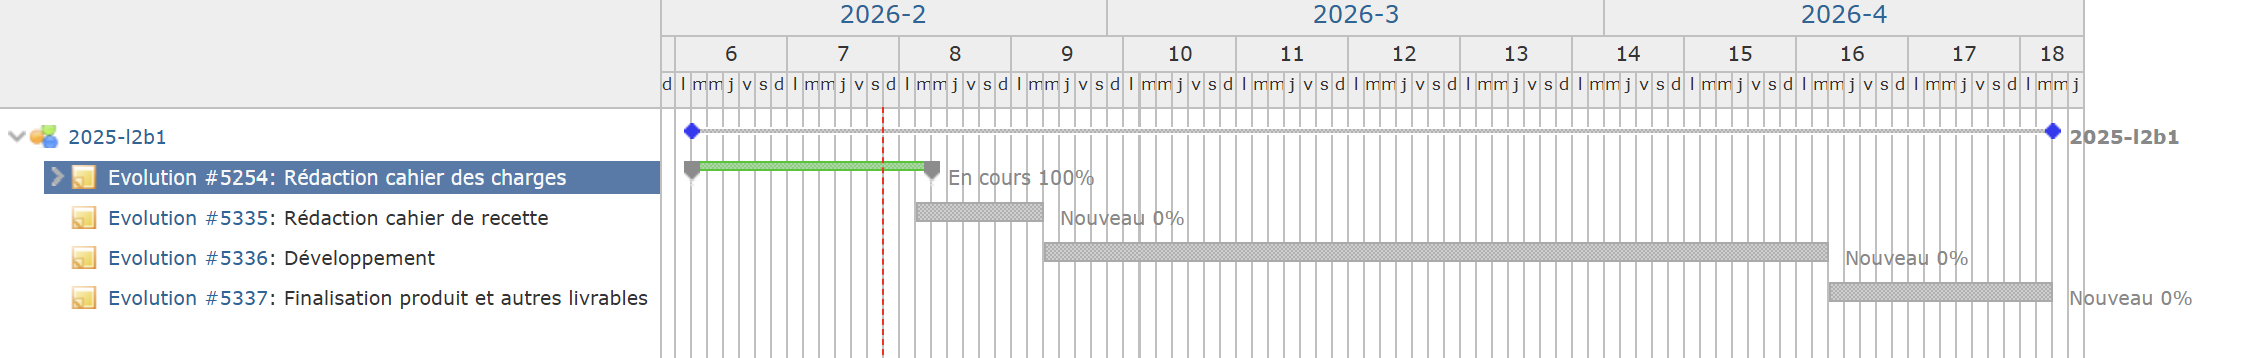
\includegraphics[width=1\textwidth]{diagramme_gantt_general.png}
    \caption{Diagramme de Gantt}
\end{figure}

\section{Ressources}
\label{rssrc}
\subsection{Ressources matérielles}
\begin{itemize}
    \item Accès aux salles informatiques de l’université.
    \item Accès au réseau Internet de l’établissement.
    \item Mise à disposition du sujet du projet et des consignes associées.
    \item Autorisation d’utiliser des jeux de données publics.
\end{itemize}

\subsection{Ressources humaines}
\begin{itemize}
    \item Une équipe de 4 développeurs (backend, frontend, intégration, documentation).
    \item Un encadrant pédagogique assurant le suivi du projet, l’accompagnement méthodologique et sa disponibilité ponctuelle pour répondre aux questions fonctionnelles et valider les livrables.
\end{itemize}


\chapter*{Annexes}
\addcontentsline{toc}{chapter}{Annexes}
\setcounter{figure}{0} % On recommence le comptage des images à 0
\renewcommand{\thefigure}{A.\arabic{figure}} % On préfixe par "A" (Annexe)
\setcounter{table}{0} % On recommence le comptage des tableaux à 0
\renewcommand{\thetable}{A.\arabic{table}} % On préfixe par "A"

\begin{enumerate}[label=A.\arabic*, leftmargin=1.7cm]
    \item Maquette du site web :
    \label{SW}
        \begin{figure}[h]
            \centering
              % Première image (à gauche)
            \begin{minipage}{0.48\textwidth}
                \centering
                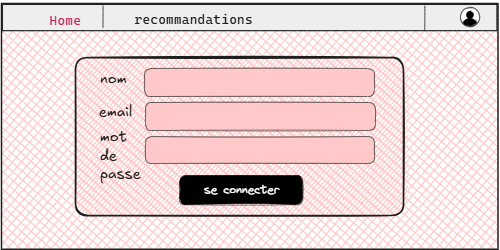
\includegraphics[width=\textwidth]{connexion.png}
            \end{minipage}
            \hfill
              % Deuxième image (à droite)
            \begin{minipage}{0.48\textwidth}
                \centering
                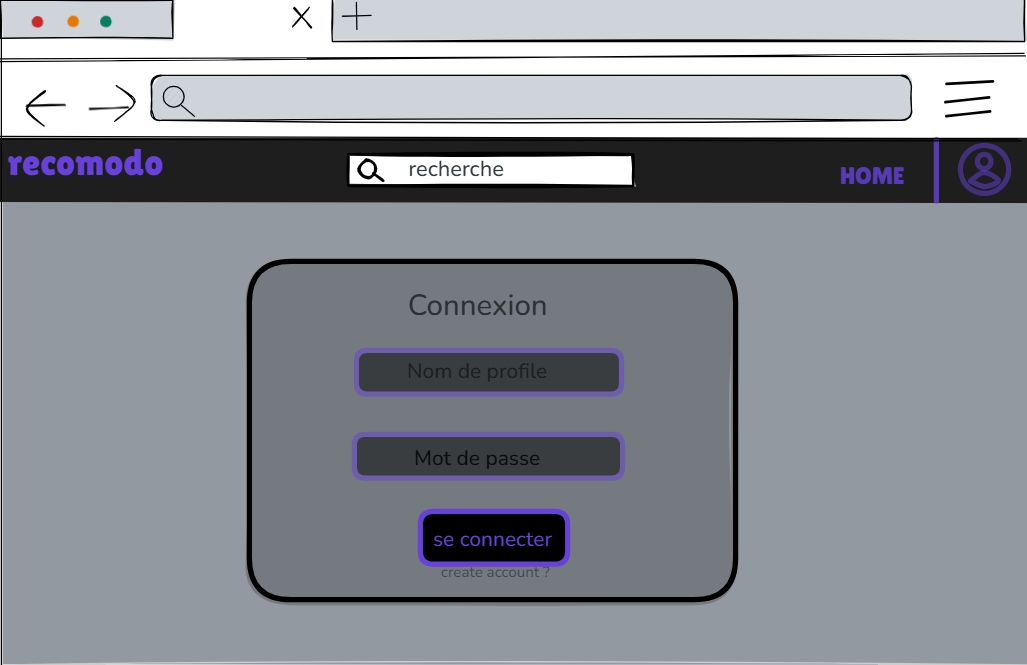
\includegraphics[width=0.9\textwidth]{page_connexion.jpeg}
            \end{minipage}
            \caption{Aperçu de l'authentification}
            \label{fig:1}
        \end{figure}
    
        \begin{figure}[h]
            \centering
              % Première image (à gauche)
            \begin{minipage}{0.48\textwidth}
                \centering
                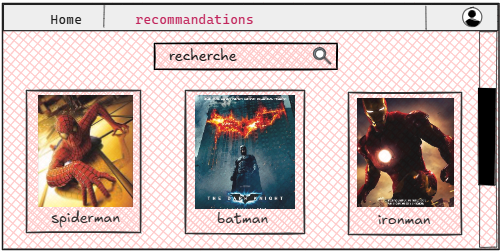
\includegraphics[width=\textwidth]{films.png}
            \end{minipage}
            \hfill
              % Deuxième image (à droite)
            \begin{minipage}{0.48\textwidth}
                \centering
                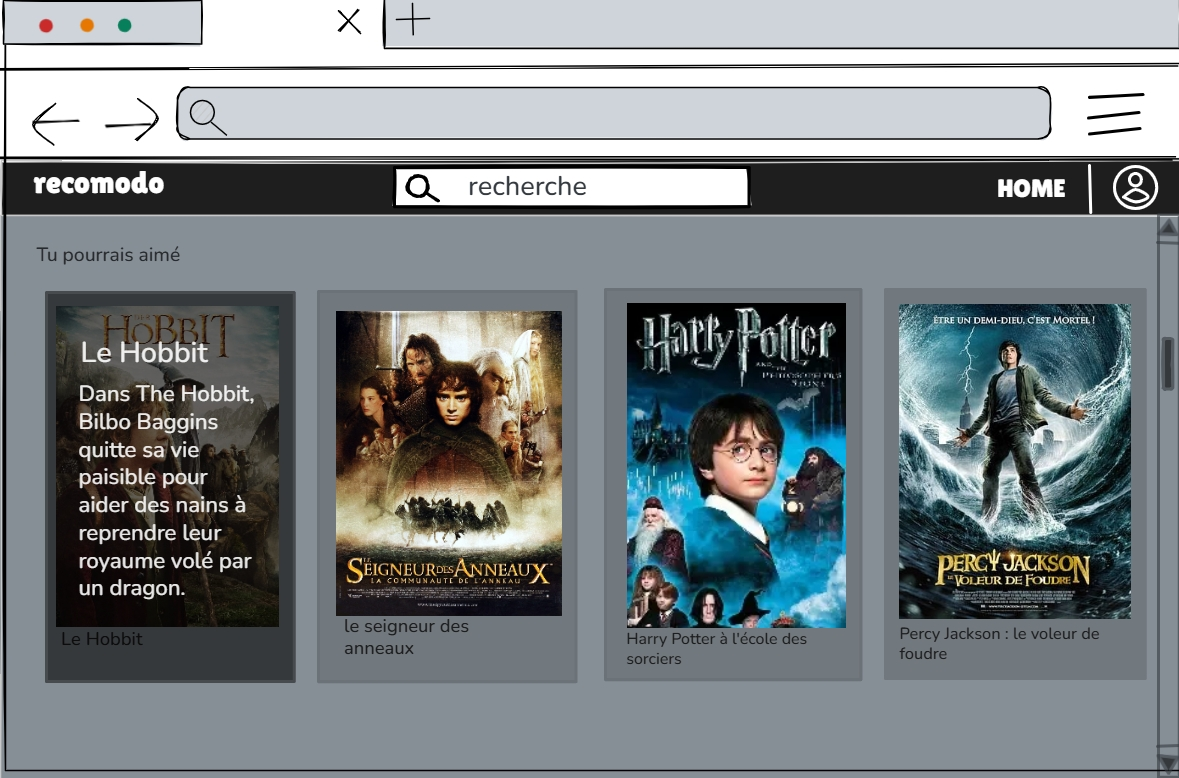
\includegraphics[width=0.9\textwidth]{maquette_hover.jpeg}
            \end{minipage}
            \caption{Aperçu de la liste de films}
        \end{figure}
    
        \begin{figure}[h]
            \centering
              % Première image (à gauche)
            \begin{minipage}{0.48\textwidth}
                \centering
                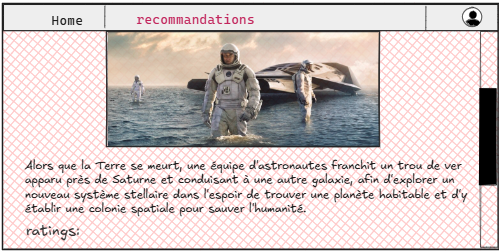
\includegraphics[width=\textwidth]{film.png}
            \end{minipage}
            \hfill
              % Deuxième image (à droite)
            \begin{minipage}{0.48\textwidth}
                \centering
                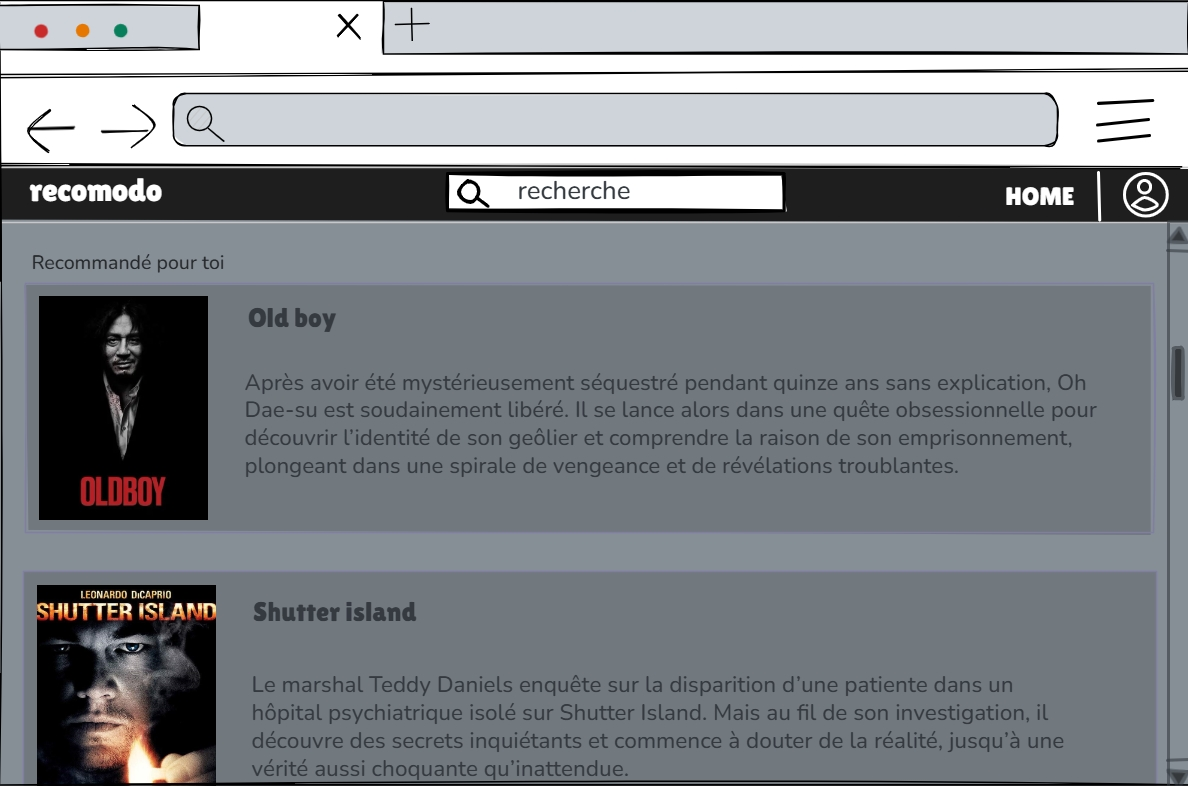
\includegraphics[width=0.9\textwidth]{maquette_resume.jpeg}
            \end{minipage}
            \caption{Aperçu de la page de résumé}
        \end{figure}
    
    \newpage
    \label{JD2}
    \item Le jeu de données que nous avons choisi est libre de droit. Il contient une liste de 45 000 films ainsi que 26 millions de notes.\\
    NB : le jeu de données contient des versions small des fichiers \texttt{links.csv} et \texttt{rating.csv} qui contiennent respectivement 9 000 films et 100 000 notes pour ces 9 000 films.
    
    Voici les schémas des différents fichiers :

        \begin{table}[h]
            \centering
            \small
            \begin{tabular}{@{}ll@{}}
                \toprule
                \textbf{Propriétés (Colonnes)} & \textbf{Type / Description} \\
                \midrule
                \textbf{adult} & (Bool)\\
                \textbf{belong\_to\_collection} & id, name, poster\_path, backdrop\_path\\
                \textbf{budget} & (Integer)\\
                \textbf{genres} & id, name\\
                \textbf{homepage} & (String)\\
                \textbf{id} & (Integer)\\
                \textbf{imdb\_id} & (String)\\
                \textbf{original\_language} & (String)\\
                \textbf{original\_title} & (String)\\
                \textbf{overview} & (String)\\
                \textbf{popularity} & (Float)\\
                \textbf{poster\_path} & (String)\\
                \textbf{production\_companies} & name, id\\
                \textbf{production\_countries} & iso\_3166\_1, name\\
                \textbf{release\_date} & (Date)\\
                \textbf{revenue} & (Integer)\\
                \textbf{runtime} & (Float)\\
                \textbf{spoken\_languages} & iso\_639\_1, name \\
                \textbf{status} & (String)\\
                \textbf{tagline} & (String)\\
                \textbf{title} & (String)\\
                \textbf{video} & (Bool)\\
                \textbf{vote\_average} & (Float)\\
                \textbf{vote\_count} & (Integer)\\
                \bottomrule
            \end{tabular}
            \caption{Structure du fichier \texttt{movies\_metadata.csv}}
        \end{table}

        \begin{table}[h]
            \centering
            \begin{tabular}{@{}ll@{}}
                \toprule
                \textbf{Propriétés (Colonnes)} & \textbf{Type/Description} \\
                \midrule
                \textbf{movieId} & (Integer) \\
                \textbf{imdbId} & (Integer) \\
                \textbf{tmdbId} & (Integer) \\
                \bottomrule
            \end{tabular}
            \caption{Structure du fichier \texttt{links.csv}}
        \end{table}
    
        \begin{table}[h]
            \centering
            \begin{tabular}{@{}llll@{}}
                \toprule
                \textbf{Propriétés (Colonnes)} & \textbf{Cast} & \textbf{Crew} & \textbf{Id} \\
                \midrule
                \textbf{Type/Description} & cast\_id & credit\_id & (Integer) \\
                &character & department \\
                &credit\_id & gender \\
                &gender & id \\
                &id & job \\
                &name & name \\
                &order & profile\_path \\
                &profile\_path \\
                \bottomrule
            \end{tabular}
            \caption{Structure du fichier \texttt{credit.csv}}
        \end{table}

        \begin{table}[!h]
            \centering
            \begin{tabular}[t]{@{}ll@{}}
                \toprule
                \textbf{Propriété (Colonnes)} & \textbf{Type/Description} \\
                \midrule
                \textbf{id} & (Integer)\\
                \textbf{keywords} & id, name \\
                \bottomrule
            \end{tabular}
            \caption{Structure du fichier \texttt{keywords.csv}}
        \end{table}
        
\end{enumerate}


\chapter*{Glossaire}
\addcontentsline{toc}{chapter}{Glossaire}
\label{BE2}
\begin{itemize}
    \item \underline{Algorithme} : Un algorithme peut s'apparenter à une recette de cuisine, il s'agit d'un ensemble fini d'instructions détaillées permettant de résoudre un problème ou faire une tâche.\\
    \underline{NB} : Dans notre cas, nous utiliserons un algorithme de recommandation, qui permet de proposer des contenus pertinents à un utilisateur.
    
    \item \underline{Backend} : Le backend est la partie invisible, qui gère le fonctionnement interne du produit (par exemple : les données).
    
    \item \underline{Bug} : Un bug est un défaut de conception d'un programme informatique à l'origine d'un dysfonctionnement.
    
    \item \underline{Comma Separated Values (CSV)} : Un fichier CSV est un fichier texte dont le format spécifique permet d'enregistrer des données structurées sous forme de tableau.
    
    \item \underline{La Forge} : La forge est une plateforme de développement collaboratif utilisée principalement pour la gestion de projets logiciels.
    
    \item \underline{Framework} : Un framework est une structure prête à être utilisée pour développer un logiciel, il contient des outils et des bibliothèques.
    
    \item \underline{Frontend} : Le frontend est la partie visible du site web, c'est ce avec quoi l'utilisateur interagit directement.
    
    \item \underline{Jeu de données} : Un jeu de données est un ensemble structuré de données. 
    
    \item \underline{Intégration} : L'intégration est le fait d'assembler plusieurs modules, composants ou systèmes afin qu'ils fonctionnent correctement ensemble.
    
    \item \underline{Interface web} : Une interface web est une interface  à laquelle on accède et qui s'affiche grâce à un navigateur web, qui permet un dialogue entre l'utilisateur et le système.
    
    \item \underline{Similarité} : (dans le cadre de la recommandation) La similarité permet de mesurer à quel point deux éléments se ressemblent, elle est souvent exprimée sous forme de note.
    
    \item \underline{Site web} : Un site web est un ensemble de pages web qui peuvent être consultées en suivant des hyperliens à l'intérieur du site

    \item \underline{Subversion (SVN)} : SVN est un gestionnaire de version de code source.

    \item \underline{Système de recommandation} : Un système de recommandation est un système qui permet de proposer des contenus ou des produits en fonction de ses préférences.
    
\end{itemize}




\chapter*{Références}
\addcontentsline{toc}{chapter}{Références}
\begin{itemize}
    \item Rounak,  Banik. « The Movies Dataset ». 2018,\\ \url{https://www.kaggle.com/datasets/rounakbanik/the-movies-dataset/data?select=credits.csv.}
    
    \item Saporta, Gilbert. Algorithmes de recommandation. Éditions Technip, 2022, p. 247. cnam.hal.science,\\ \url{https://cnam.hal.science/hal-03696281}.
    \item Tushar Jain. un rapport de projet sur système de recommandation de films,
    \begin{flushleft}\url{https://fr.scribd.com/document/821410413/Rapport-de-projet-de-recommandation-de-films}\end{flushleft}
    \item Romero, Julien. « Systèmes de recommandation »,\\
    \url{https://www-inf.telecom-sudparis.eu/COURS/CSC4538/Supports/cours/recommender.pdf}
    \item Rakotomalala, Ricco. « Filtrage collaboratif et Système de recommandation ».\\
    \url{https://eric.univ-lyon2.fr/ricco/cours/slides/WM.B%20-%20Filtrage%20Collaboratif%20-%20Recommandation.pdf}
    \item Fournier-S’niehotta, Raphaël. « Systèmes de recommandation ».\\
    \url{https://cedric.cnam.fr/vertigo/cours/RCP217/docs/RCP217-RecSys1.pdf}


    \item « AWS Amplify ». Amazon Web Services, Inc.,\\ \url{https://aws.amazon.com/fr/amplify/. Consulté le 15 février 2026}
    \item « AWS Amplify | Applications Web et mobiles extensibles | Amazon Web Services ». Amazon Web Services, Inc.,\\ \url{https://aws.amazon.com/fr/amplify/extensibility/. Consulté le 15 février 2026}

    \item Cahier des charges : comment le rédiger + modèle (8 étapes). 23 janvier 2026,\\
    \url{https://blog-gestion-de-projet.com/cahier-des-charges-projet/}
    \item Maîtrise d’œuvre \& Maîtrise d’ouvrage: quelles différences? 26 février 2021,\\
    \url{https://blog-gestion-de-projet.com/maitrise-doeuvre/}
    \item «Modèle cahier des charges site internet à télécharger». la fabrique du net,\\
    \url{https://www.lafabriquedunet.fr/modele/exemple-cahier-des-charges-site-internet/}

    \item Un exemple de site de recommandation : MovieLens,\\
    \url{https://movielens.org/profile}
\end{itemize}

\chapter*{Index}
\addcontentsline{toc}{chapter}{Index}
\begin{itemize}
    \item Acceptabilité \pageref{acceptabilité}
    \item Algorithme de recommandation \pageref{algorec},\pageref{BE2}
    \item AWS Amplify \pageref{cont1}
    \item Backend \pageref{BE1},\pageref{BE2}
    \item Bug \pageref{BE2}
    \item Contraintes \pageref{cont1}
    \item CSV \pageref{JD2},\pageref{BE2}
    \item Fonctionnalités \pageref{fnct}
    \item La Forge \pageref{cont2},\pageref{BE2}
    \item Framework \pageref{BE2}
    \item Frontend \pageref{BE2}
    \item Intégration \pageref{BE2}
    \item Interface web \pageref{JD1},\pageref{fnct},\pageref{BE2}
    \item Jeu de données \pageref{JD1},\pageref{JD2}
    \item Planification \pageref{plan}
    \item Recommandation \pageref{algorec}
    \item Ressources \pageref{rssrc}
    \item Site web \pageref{SW},\pageref{BE2}
    \item SVN \pageref{cont2},\pageref{BE2}
    \item Système de recommandation \pageref{algorec},\pageref{BE2}
    
\end{itemize}

\end{document}